\documentclass{PHlab-thesis}
\usepackage{amsmath}
\usepackage{amsfonts} 
\usepackage{graphicx}
\usepackage{algpseudocode}
\usepackage{algorithm}
\usepackage{subfigure}
\addbibresource{thesis.bib}

\newcommand*\Department中文{資訊工程學研究所}
\newcommand*\Department英文{Institute of Computer Science and Information Engineering}

\newcommand*\ThesisTitle中文{搜尋最適合亞硫酸氫鹽測序數據之基因組變異與胞嘧啶甲基化狀態的組合 — 基於 EAGLE 變異點評估器程式碼庫之案例研究}
\newcommand*\ThesisTitle英文{Searching for combinations of genome variants and cytosine methylation state which best fit bisulfite sequencing data — a case study using the EAGLE variant evaluator program code base
}
% \newcommand*\ThesisNote中文{示例:其實徐翡曼是東京大學畢業的博士}% For real thesis omit, or use {初稿} etc.
% \newcommand*\ThesisNote英文{Just an example.  Fei-Man actually graduated from Tokyo Univ.}% For real thesis omit, or use {draft} etc.

\newcommand*\Student中文{張恆霖}
\newcommand*\Student英文{Heng-lin Chang}

\newcommand*\Advisor中文{賀保羅}
\newcommand*\Advisor英文{Paul Horton}

%% 果有共同指導老師可以用:
%% \newcommand*\CoAdvisorA中文{}
%% \newcommand*\CoAdvisorA英文{}
%% \newcommand*\CoAdvisorB中文{}
%% \newcommand*\CoAdvisorB英文{}


\newcommand*\YearMonth英文{July, 2022}
\newcommand*\YearMonth中文{111年7月}

\pagestyle{fancy}% Use fancyhdr
\begin{document}


\newcommand*\Keywords英文{Genomics, Methylation, Bisulfite Sequencing, Probability Model}
\newcommand*\Abstract英文{%
DNA methylation~\cite{moore2013dna} is a form of chemical modification of DNA that affects the genetic expression of DNA without changing the sequence, which is part of the so-called epigenetic code, and it is also part of an epigenetic mechanism. The process of DNA methylation is the articulation of the Methyl group at the  5' carbon position of the cytosine ring~\cite{barker1964crystal}, and this methylation is articulated in the cytosine 5' direction, which is more common in all vertebrates.
\par The occurrence of DNA methylation leads to a decrease in the transcriptional rate of that region of the gene, which means that it may inhibit the associated production of proteins, a phenomenon also known as Gene silencing, which in turn renders it non-functional and plays a key role in development and cancer. In human cells, about 1\% of the bases are methylated. In mature cells, DNA methylation usually occurs at the CpG dinucleotide, and about 80\% of the CpG sites in human genes may be methylated, but some specific regions are not methylated, such as dense cytosine and guanine. We call that the CpG island. This is associated with promoters in 56\% of mammalian genes, which contain all widely expressed genes. Therefore, for humans, the study of methylation in mammals is of great relevance to the study of diseases or specific physiological phenotypes.
\par In our study, we extended the EAGLE~\cite{kuo2018eagle} model for calculating the probability of variation in an organism to evaluate the probability of methylation at the cytosine site in the gene sequence of an organism. Our approach is to emulate EAGLE by giving two hypothetical sequences, a hypothetical Reference sequence, and a hypothetical Alternative sequence. First, we evaluate the likelihood score of the variant to the organism by referring to the variant data and use the sites with a higher likelihood of variation to modify the reference genome sequence, so that we can obtain a reference genome with the replacement of the possible variant sites, call modified reference. Then, we took the sequences that were assumed to be methylated at all CpG sites as the reference genome, then added the sequences that were assumed to be methylated at each site as alternative genomic sequences to the generative probability model, and calculated the highest probability scores of methylation at each CpG site by the Greedy algorithm. In the calculation process, because our data source is the data from bisulfite sequencing~\cite{krueger2012dna}, we have to take into account the different situations from the biological sequence information of positive and negative strands. In the output, the higher the probability of deamination combination at the site of the sequence, the higher the degree of methylation of the individual sequence at that site. In the EAGLE-METH design framework, users can infer the likelihood of CpG site methylation by inputting the information of an individual after bisulfite sequencing and polymerase chain reaction.
\par In our experiments, the highest probability scores for each CpG site were selected by our designed probability model and compared with the simulated methylation experimental data. We could almost predict most of the simulated CpG sites, and the probability scores of methylated CpG sites given by EAGLE-METH were mostly consistent with the actual data.
}


\newcommand*\Keywords中文{基因組、甲基化、亞硫酸鹽定序、機率模型}
\newcommand*\Abstract中文{%
\qquad 近幾年以來,在基因表關遺傳學的研究領域當中,很重要的一塊主題,就是 DNA 的甲基化現象。DNA 甲基化~\cite{moore2013dna}是 DNA 化學修飾的一種形式,它能影響 DNA 序列,在不改變序列的情況下,改變其序列原本會產生的遺傳表現,就是所謂的表觀遺傳編碼 (epigenetic code)。DNA 甲基化的發生會導致基因該區段的轉錄作用率降低,意即可能抑制蛋白質的相關生成,而這種現象又稱為基因靜默 (Gene silencing),進而使其失去功能,在影響發育與癌症中扮演關鍵作用 。在人類的細胞中,大約有1\%的鹼基是發生甲基化作用的,在一般成熟的細胞當中,DNA 甲基化通常發生於 CpG 雙核甘酸 (CpG dinucleotide),在人類的基因中,大約80\%左右的 CpG 位點可能都發生甲基化,但某些特定區域則未發生甲基化,例如密集的胞嘧啶和鳥嘌呤,也就是所謂的 CpG島 (CpG island)。而這與包含所有廣泛表達基因在內的50\%的哺乳動物基因中的啟動子有關 。因此對人類來說,研究哺乳動物之甲基化程度的現象,對於探討疾病或是特定生理表徵有著龐大的關係\\ \qquad 在我們的研究中,我們參考了 EAGLE~\cite{kuo2018eagle} 的作法,將 EAGLE 計算生物體變異的生成機率模型,延伸應用至探討生物體基因序列中,胞嘧啶位點發生甲基化之可能性進行評估。我們的做法是模仿 EAGLE,分別給定兩種假設序列,分別為假設的參考基因組序列 (Reference sequence) 以及假設的替代基因組序列 (Alternative sequence) 。首先,我們參考變異資料,先評估該變異資料對生物體的可能性評分,將評分後變異可能性發生較高的位點用來修改參考基因組序列,因此我們能得到一組已經將變異可能發生位點替換後的參考基因組 。再來,我們將所有 CpG 位點假設皆已發生甲基化的序列當作參考基因組,接著分別將每個位點各自假設發生甲基化的序列當作替代基因組序列各自加入生成機率模型,並藉由貪婪演算法,分別計算各個 CpG 位點發生甲基化之最高可能性評估分數,在計算過程中,因為我們的資料來源為經過亞硫酸鹽定序~\cite{krueger2012dna}之資料,故在計算過程中,須考慮到來自生物序列資訊正股反股不同之情況。在輸出的結果中,若是原生物個體序列的位點其脫氨組合的可能性越高,則代表該生物個體序列在該位點傾向發生甲基化的程度越高 。在 EAGLE-METH 的設計架構中,使用者可以透過輸入經過亞硫酸鹽定序以及聚合酶連鎖反應後的個體資訊,來推斷生物個體 CpG 位點型甲基化發生的可能性評估。\\ \qquad 在我們的實驗中,透過我們設計的生成機率模型,經由模型的計算,挑選出各個 CpG 位點可能發生甲基化之最高可能性分數,與模擬的甲基化實驗數據做比較,我們幾乎可以推測大部分模擬發生甲基化的 CpG 位點,EAGLE-METH 給予之甲基化 CpG 位點的可能性分數,也大部分符合實際資料。
}

\newcommand*\Acknowledgements{%
感謝我...}



\newcommand*\SelectFontsize[2]{\fontsize{#1}{#1}\selectfont\mdseries#2\par}
\newcommand*\SelectFontsizeBF[2]{\fontsize{#1}{#1}\selectfont\bfseries#2\par}
\newcommand*\SignatureRule[1][6]{\rule{#1cm}{0.3mm}}
\newcommand*\AddToContents[1]{\newpage\phantomsection\addcontentsline{toc}{chapter}{#1}}

\doublespace
\pagenumbering{gobble}
\renewcommand{\thefootnote}{\fnsymbol{footnote}}


\begin{center}
\vspace{2cm}
\SelectFontsizeBF{24}{%
\University中文\Department中文\\
\學位 論文}

\vfill
\SelectFontsizeBF{24}{\ThesisTitle中文}
\ifdefined\ThesisNote中文
\SelectFontsize{22}{\textit{\ThesisNote中文}}
\fi

\vspace{5mm}
\SelectFontsizeBF{22}{\ThesisTitle英文}
\ifdefined\ThesisNote英文
\SelectFontsize{20}{\textit{\ThesisNote英文}}
\fi

\vfill

\begin{minipage}{\linewidth}
{\setlength\tabcolsep{0pt}
%
\begin{tabular}{ Wr{5em} Wl{6em} Wr{5em} wl{7em} }
研究生:   & ~~\Student中文  &      Student: & ~~\Student英文\\
指導老師: & ~~\Advisor中文  &      Advisor: & ~~\Advisor英文\\
\ifdefined\CoAdvisorA中文
共同指導: & ~~\CoAdvisorA中文 &   Co-Advisor: & ~~\CoAdvisorA英文\\
\fi
\ifdefined\CoAdvisorB中文
         & ~~\CoAdvisorB中文 &   Co-Advisor: & ~~\CoAdvisorB英文\\
\fi
\end{tabular}
}
\end{minipage}

\vfill
\SelectFontsize{18}{%
National Cheng Kung University,\\
Tainan, Taiwan, R.O.C.\\
Thesis for \ifdef\PhD{Doctor of Philosophy}{Master of Science} Degree\\
\YearMonth英文}

\vfill
\SelectFontsize{20}{中華民國\YearMonth中文}
\end{center}



\ifdefined\optCommittee
\newpage
\begin{center}
\vspace{1cm}
\SelectFontsizeBF{24}{%
\University中文\Department中文\\
\學位 論文}
\vfill
\SelectFontsizeBF{20}{\ThesisTitle中文}
\end{center}

\vfill
\SelectFontsize{20}{%
\noindent 研究生:\Student中文\\
本論文業經審查及口試合格特此證明}


\begin{center}
\SelectFontsize{18pt}{論文考試委員}
\vfill
\SignatureRule \hspace*{1cm} \SignatureRule
\vfill

\SignatureRule \hspace*{1cm} \SignatureRule
\vfill

指導教授:\SignatureRule[8]
\vfill
  所長:\SignatureRule[8]

\vfill
\SelectFontsize{18}{中華民國 \hspace{2em} 年 \hspace{2em} 月 \hspace{2em} 日}
\end{center}


\newpage
\begin{center}
\vspace{1cm}
\SelectFontsize{18}{\University英文, \Department英文}
\SelectFontsize{19}{\ifdef\PhD{Ph.D.}{Master's} Degree Thesis}

\vfill
\SelectFontsizeBF{20}{\ThesisTitle英文}
\end{center}

\vfill
\SelectFontsize{18}{Student: \Student英文}

\SelectFontsize{18}{%
A thesis submitted to the graduate division in partial fulfillment of the requirement for the degree of
\ifdef\PhD{Doctor of \mbox{Philosophy}}{Master of Science}.
}

\vfill
\begin{center}
\SelectFontsize{18}{Approved by}

\vfill
\SignatureRule \hspace*{1cm} \SignatureRule

\vfill
\SignatureRule \hspace*{1cm} \SignatureRule

\vfill
Advisor: \SignatureRule[8]

\vfill
Chairman: \SignatureRule[8]

\vfill
\SelectFontsize{18}{\YearMonth英文}
\vspace*{20pt}
\end{center}
\fi% optCommittee


\AddToContents{中文摘要}
\setcounter{page}{1}
\pagenumbering{roman}


\begin{center}
\SelectFontsizeBF{24}{\ThesisTitle中文}

\vspace{4mm}
\SelectFontsize{18}{\Student中文\footnote[1]{學生} ~ \Advisor中文\footnote[2]{指導教授}}

\vspace{5mm}
\SelectFontsize{20}{國立成功大學\Department中文}

\vspace{12mm}
\makebox[2.7cm][c]{\SelectFontsizeBF{22}{摘要}}

\vspace{4mm}
\SelectFontsize{16}{\Abstract中文}

\vspace{4mm}
\begin{flushleft}
\SelectFontsize{16}{\textbf{關鍵詞:} \Keywords中文}
\end{flushleft}
\end{center}


\AddToContents{Abstract}
\begin{center}
\SelectFontsizeBF{22}{\ThesisTitle英文}

\vspace{4mm}
\SelectFontsize{18}{\Student英文\footnote[1]{Student} ~ \Advisor英文\footnote[2]{Advisor}}

\vspace{4mm}
\SelectFontsize{16}{\Department英文, National Cheng Kung University}

\vspace{12mm}
\SelectFontsizeBF{20}{Abstract}

\vspace{4mm}
\SelectFontsize{14}{\Abstract英文}
\end{center}

\vspace{4mm}
\begin{flushleft}
\SelectFontsize{16}{\textbf{Keywords:} \Keywords英文}
\end{flushleft}



\AddToContents{誌謝}
\begin{center}\SelectFontsizeBF{24}{誌謝}\end{center}

\vspace{4mm}
\Acknowledgements



\renewcommand{\contentsname}{CONTENTS}
\AddToContents{Contents}
\tableofcontents


\AddToContents{List of Tables}
\listoftables


\AddToContents{List of Figures}
\listoffigures
% 封面頁, 口委中英文簽名單, 誌謝, 中英文摘要, 論文目錄, 圖表目錄


%────────────────────  List of Symbols  ────────────────────
\renewcommand\nomgroup[1]{%
  \item[\bfseries
  \ifstrequal{#1}{A}{General}{%
  \ifstrequal{#1}{Z}{Gene/Protein Names}%
  }]}

% \nomenclature[A]{$\lg$}{Logarithm base 2}
% \nomenclature[A]{KL\ Divergence}{Kullback-Liebler Divergence}
% \nomenclature[Z]{Myc}{MYC proto-oncogene}
% \nomenclature[Z]{USF-1}{Upstream stimulatory factor 1}
\nomenclature[A]{EAGLE}{Explicit Alternative Genome Likelihood Evaluator}
\nomenclature[A]{NGS}{Next Generation Sequencing}
\nomenclature[A]{DNA}{deoxyribonucleic acid}
\nomenclature[A]{bp}{base pair}
\nomenclature[A]{WGBS}{Whole Genome Bisulfite Sequencing}

\printnomenclature[5cm]

\newpage
\setcounter{page}{1}
\pagenumbering{arabic}



\chapter{Introduction}
\section{Overview}
\par The phenomenon of DNA methylation has been a topic of much discussion in recent years. If DNA methylation sites can be effectively predicted and determined, it will be possible to understand the effects of methylation on organisms and even prevent the occurrence of methylation-induced diseases. Before studying our experiments, we first studied EAGLE (Explicit Alternative Genome Likelihood Evaluator), a research project that developed a method for evaluating the degree to which sequencing data supports a given candidate genome variant. EAGLE incorporates candidate variants into explicit hypotheses about the individual’s genome, and then computes the probability of the observed data (the sequencing reads) under each hypothesis.
\par We have extended the idea of EAGLE by simulating its method of calculating variant evaluation to DNA methylation evaluation. We have created a tool that can evaluate the probability of occurrence of DNA methylation sites and retain the probability of variant evaluation, which we call EAGLE-METH.

\section{Motivation}
\par With the advancement of technology, molecular biology is advancing rapidly and there is a breakthrough in genome sequencing technology, the Next Generation Sequencing (NGS), which has a huge impact on biology. Unlike the early Sanger sequencing technology, which took about 10 years and was done by six countries, only 3 billion human bases were solved. With today's NGS technology, this can be done in a matter of days. When using Sanger for genome sequencing, the target gene has to be amplified one by one, each sequence is about 1000bp long, and then compared and assembled after sequencing, which is a tedious process, time-consuming, and costly. The NGS technology is to cut the genome into small fragments and connect them to adapters, and then perform rapid and high-throughput sequencing with the help of material science and imaging systems. 
\par DNA methylation is one of the most important topics in NGS research. DNA methylation has a certain degree of influence on the genetic performance of vertebrates. And for mammals, the occurrence of methylation may lead to adverse diseases or even cancer. Therefore, after studying the generative probabilistic model (GPM) of genomic variation in EAGLE, we have a new idea to extend the approach of EAGLE and develop a GPM as a basic computational approach to calculate the degree of cytosine methylation in sequencing data. Thus allowing us to determine the occurrence of methylation more effectively, and help to explore the impact of methylation on us for disease prevention and treatment of cancer.

\section{Research framework}
\par The organizational structure of our paper is as follows: In chapter 1, we introduce the research background, the overview of EAGLE-METH, the technology, and the issue of methylation in biology, including sequencing technology, how methylation affects human gene expression, and problems of methylation caused. Thence, we decided to research EAGLE and extend it to evaluate the sequence's methylation level. Chapter two, we introduce the background knowledge of this study, including the previous studies: EAGLE, introduction to methylation, bisulfite sequencing technique, and some data types. Chapter three introduces some related work and the EAGLE-METH framework and practices. Chapter four introduces the experiments in this study, the experimental environment using those tools, and how different cases are configured. In chapter five, which is also the last chapter, we conclude this study, EAGLE-METH, and propose those problems that still need to be improved in the future.

\chapter{Background}
\section{EAGLE}
EAGLE is our previous research, which is a method to calculate genome variant likelihood.EAGLE incorporates candidate variants into explicit hypotheses about the individual’s genome, and then computes the probability of the observed data (the sequencing reads) under each hypothesis. First of all, you need to give three different inputs: the reference genome sequence, the called variant candidates in a vcf file and reads information(see Figure \ref{fig:eagle_workflow}). In EAGLE, we will evaluate candidate genome variant amounts by considering two hypothetical genome sequences, respectively, the reference sequence, and the alternative sequence. With the given data, we could obtain the quality of candidate variants by examining whether the reads better support the hypothesis that they were sequenced from the reference genome, or rather being more likely to be sequenced from an alternative sequence consisting of the candidate variants, indicating a higher probability that the candidate variants are present.
Therefore, we applied the eagle extension to our EAGLE-METH research. We simulated the probability model of EAGLE generation and changed its calculation mode. The bisulfite sequence considering forward strand and reverse strand shares are added. When read from the forward strand, C to T must be taken into account, and when read from the reverse strand, G to A must be taken into account. We will also give two hypothesis sequences, respectively, reference sequence and alternative sequences. The detailed system architecture will be explained in Method.

\begin{figure}[h]
    \centering
    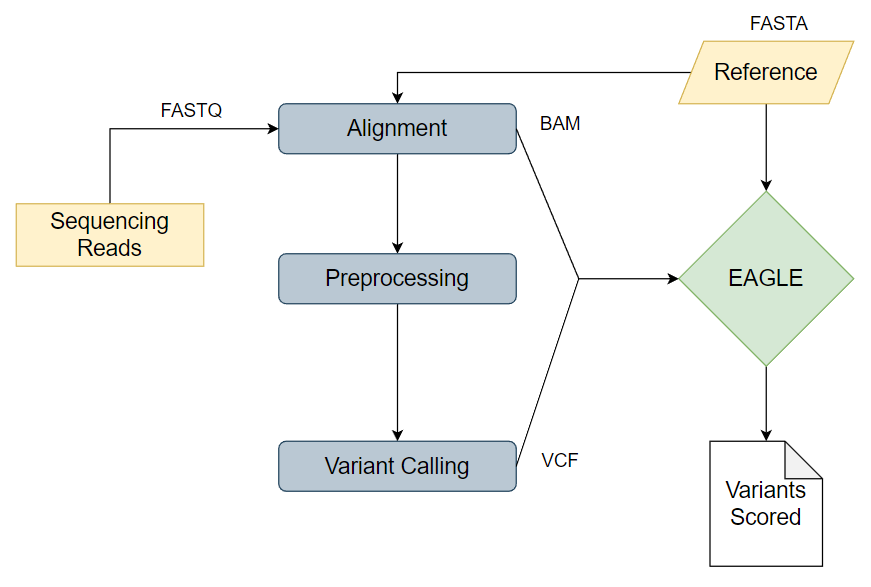
\includegraphics[scale=0.8]{figures/eagle_workflow.PNG}
    \caption{A high level overview of the EAGLE workflow}
    \label{fig:eagle_workflow}
\end{figure}

\par In brief, EAGLE will use the read information that is aligned to the specific region reference sequence position according to the variant calling file.EAGLE divides different variants into the different variant sets and combines them, considers all variant combinations, and then replaces the corresponding position of the reference, generates an alternative sequence, and performs calculations.Therefore, we applied the eagle extension to our EAGLE-METH research. We simulated the probability model of EAGLE generation and changed its calculation mode. The bisulfite sequence considering forward strand and reverse strand shares are added. When read from the forward strand, C to T must be taken into account, and when read from the reverse strand, G to A must be taken into account. We will also give two hypothesis sequences, respectively, reference sequence and alternative sequences. The detailed system architecture will be explained in Method.

\section{Methylation}
DNA methylation is a form of chemical modification of DNA that can alter gene expression without altering the DNA sequence. As part of the epigenetic code, it is an epigenetic mechanism. The process of DNA methylation adds methyl groups to DNA molecules, such as on the 5' carbon of the cytosine ring (Figure \ref{fig:methylation}).DNA methylation constitutes the most stable type of epigenetic modification modulating the transcriptional plasticity of mammalian genomes.

\begin{figure}[h]
  \centering
  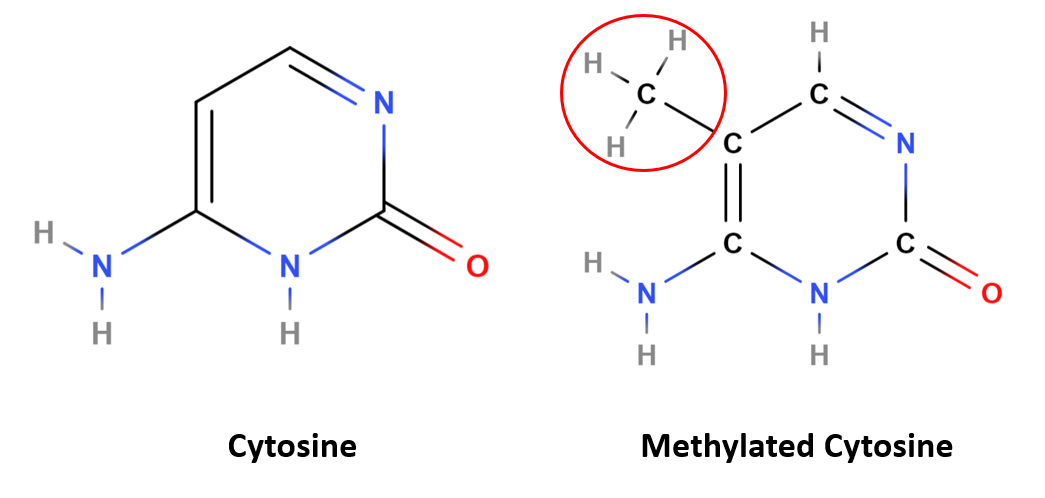
\includegraphics[scale=0.8]{figures/1.PNG}
  \caption{Left: normal cytosion, right: DNA methylation occurred}
  \label{fig:methylation}
\end{figure}

\par In general, in mature somatic tissues, methylation usually occurs at the CpG dinucleotide site, where the base sequence appears as cytosine followed by guanine. It is worth noting that 70-80\% of cytosine at CpG sites is methylated, but most of the methylation occurs outside the CpG island. CpG island refers to a region rich in CpG sites. Generally, the formal definition of a CpG island is: a fragment with a length of at least 200bp, with a CG content of more than 50\% (Figure \ref{fig:CpG_island}).
\vfill
\begin{figure}[h]
  \centering
  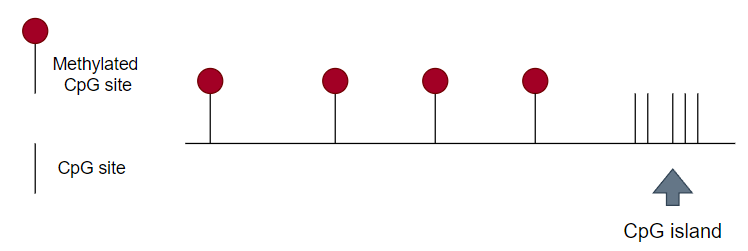
\includegraphics[scale=0.8]{figures/CpG_island.PNG}
  \caption{The CpG island}
  \label{fig:CpG_island}
\end{figure}

Benign DNA methylation helps organisms grow, while bad DNA methylation increases gene silencing (Figure \ref{fig:Gene_silencing}) and the incidence of disease .therefore, in our research, EAGLE-METH, we will focus on cytosine methylation to facilitate research and prevent the consequences of poor methylation.

\begin{figure}[h]
  \centering
  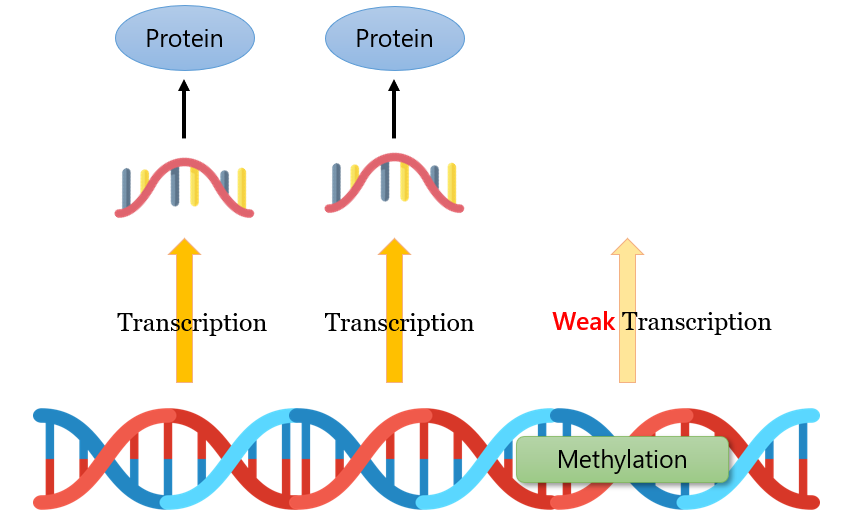
\includegraphics[scale=0.8]{figures/Gene_silencing.PNG}
  \caption{\textbf{The Gene silencing}: A phenomenon in which biological cells suppress the expression of a gene through various mechanisms of gene expression regulation}
  \label{fig:Gene_silencing}
\end{figure}

\section{Bisulfite sequencing}
In the field of DNA methylation research in the field of biology, there is an important sequencing technology, that is, bisulfite sequencing. Bisulfite sequencing~\cite{darst2010bisulfite} using next-generation sequencers yields genome-wide measurements of DNA methylation at single-nucleotide resolution. Traditional aligners are not designed for mapping bisulfite-treated reads, where the unmethylated Cs are converted to Ts. It is of great help in the field of methylation research to be able to determine the methylation sites of DNA sequences through this chemical reaction. The main process of bisulfite sequencing is divided into bisulfite and PCR. We will introduce them in the next paragraph. Nowadays, the mainstream technique used to research DNAm is the WGBS (Whole Genome Bisulfite Sequencing) and the targeted bisulfite sequencing.WGBS allows for measuring methylation in the whole human genome, and the targeted bisulfite that allows the sequence of the specific genomic regions. Both techniques belong to Next Generation Sequencing.
\subsection{Bisulfite}
Bisulfite treatment is a common chemical reaction treatment used to judge DNA methylation sites. It mainly converts the unmethylated cytosine in the sequence into uracils through bisulfite treatment cytosine, which has been methylated, is directly retained without changing, to distinguish each other~\cite{krueger2011bismark}.
\subsection{PCR}
Polymerase chain reaction (PCR) is a method used for the principle of DNA double-strand replication, nucleic acid synthesis technology that replicates specific DNA fragments in vitro. Through this technology, the target gene can be amplified in large quantities in a short time without relying on organisms such as Escherichia coli or yeast. Typical bisulfite sequencing technology includes PCR. After PCR, amplification covers the uracils from these non-methylation cytosines into thymines by a deamination process.
\subsection{Bisulfite sequencing - Example}
Give an example, as shown in Figure \ref{fig:BS_seq}. This is a double-stranded DNA fragment, and it can be seen that the position 3 site of the original forward strand (OT) is non-methylated cytosine, while the position 5 site is methylated cytosine. In addition, in the original reverse strand (OB), it can be seen that the position 1 site is non-methylated cytosine, and the position 6 site is methylated cytosine.
\par In the first step, we reacted to the two strands with bisulfite. After the reaction, we can observe that at position 3  of the forward strand, the original non-methylated cytosine has been converted into uracil, and the position 5 site of the original methylated cytosine remains unchanged as cytosine. Similarly, the position 1 site of the reverse strand is converted to uracil, while position 6 remains the same as cytosine, which is the result of bisulfite treatment.
In the second step, after the bisulfite treatment, we will do PCR. The function of PCR is to amplify the signal, that is, to copy the DNA fragments so that each DNA segment can produce a large number of the same fragments. This method is mainly to make some originally few fragments and then in the subsequent experiments, in order not to let them be ignored, we copy them and produce a large number of the same sequence fragments. Although this method can avoid a small number of sequence fragments being ignored, it may also cause some effects, such as enlarging the wrong sequences, etc. In Figure \ref{fig:BS_seq}, we show the result of PCR, there are four strands, OT, CTOT, OB, and CTOB. They are the original top, the complement of original top, the original bottom, and the complement of original bottom, respectively. We can find the result, by comparing it with original forward strand, the non-methylation cytosine that locates in the position 3 site, from uracil becomes thymine. Comparing with the position 1 site in the original reverse strand, we can see the from uracil to thymine, and so on. And we can compare with the original forward strand, the position 1 in CTOB becomes A from G.

\begin{figure}[h]
  \centering
  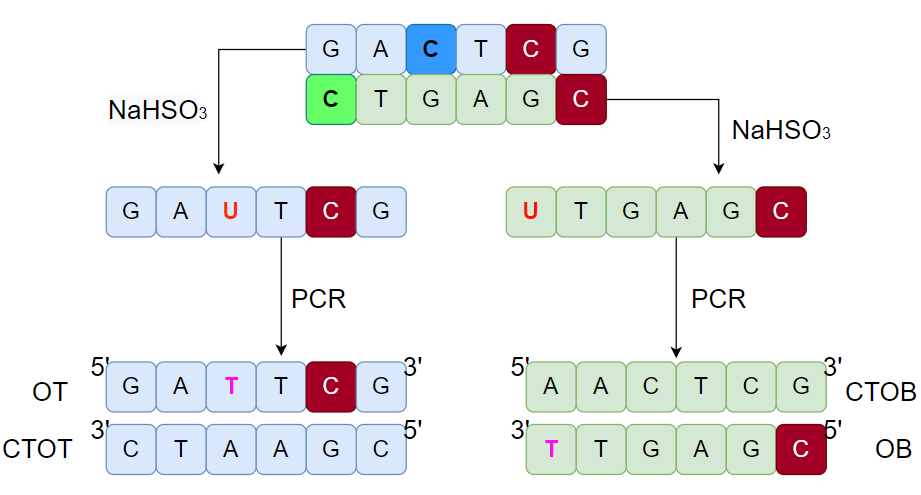
\includegraphics[scale=0.8]{figures/BS_seq.PNG}
  \caption{\textbf{Bisulfite sequencing}: blue sequence is forward strand, green sequence is reverse strand. Red cytosine is methylated. OT: the original forward strand, OB: the original reverse strand, CTOT: complement  of the original top, CTOB: complement of the original bottom. }
  \label{fig:BS_seq}
\end{figure}

\vfill
\vspace{30mm}
\section{Data format: FASTQ, FASTA, BAM, SAM}
In the field of genomic biology, it is necessary to store a large amount of genomic information before analysis and research. Therefore, the file format for storing information is relatively important. Common data storage formats are as follows: FASTA, FASTQ, SAM, BAM, VCF, etc
\par FASTA~\cite{pearson1988improved} is a text format used to record nucleic acid sequences or peptide sequences in which nucleic acids or amino acids are encoded in a single letter. This format also allows you to define names and write comments before sequences. A complete sequence in FASTA format, including the first single description line and multiple lines of sequence data. The leading half of the description line is greater than the sign (">") to distinguish it from the column. The content immediately after ">" is the identification code of the sequence, and the rest of the line is the description of the sequence.
\par FASTQ~\cite{cock2010sanger} is a file format for storing biology sequences and their sequencing quality score information. The sequence format of FASTQ can be thought of as the FASTA format plus the respective quality values of the bases.
\par SAM is the abbreviation of Sequence Alignment Map. It is a text-based format originally for storing biological sequences aligned to a reference sequence. Through the content of the SAM file, we can flexibly describe the status of various comparisons. In addition, we can also use the SAMTools provided by the author to grab specific regions, merge or sort the results of the alignment, and even grab the corresponding sequence data according to different alignment conditions, etc.
\par BAM is also a text-based format originally for storing biological sequences aligned to a reference sequence. Different from SAM, SAM is understandable by humans, and BAM is compressed into binary.
\par VCF is the abbreviation of variant calling format. It is used to record the sequenced data, which contains information about different mutations, such as SNP, indel, etc. There are 9 lines of variation information, recording CHR chromosome number, POS position, ID variation number (whether in dbSNP), REF sequence of this site on the reference gene, ALT variation sequence, QUAL sequencing quality of this sequence, whether filter passes the set screening conditions, format information, and the status of samples at this site.

\chapter{Related work and Method}
\section{Related work}
\subsection{Previous research}
In our previous study, our senior paper~\cite{ni2021} extended the application of EAGLE to bisulfite sequencing data to find unmethylation sites by using the original EAGLE model. The original reference was modified according to vcf file, and new deamination sets were added, which means the likelihood to become T from C / become A from G, the higher the likelihood of deamination sets, the lower the methylation tendency is. Unlike our method, it does not compute alternative sequence comparisons based on the hypothetical methylation CpG site.
\subsection{Burrow-Wheeler Aligner}
Burrow-Wheeler Aligner~\cite{abuin2015bigbwa} is a package for mapping DNA sequences against a large reference genome, such as the human genome. It has two major components, one for reading shorter than 150bp and the other for longer reads. It consists of three algorithms: BWA-backtrack, BWA-SW, and BWA-MEM. We used the BWA command to index the reference after executing the index function of BWA-meth ( including converting forward strand C into T and reverse strand G into A ).
\subsection{BWA-meth}
We used BWA-meth~\cite{pedersen2014fast} in our research mainly. BWA-meth is an aligner for bisulfite-treated sequences. BWA-meth is similar in function to BWA-MEM~\cite{li2013aligning}. BWA-MEM is a popular alignment tool, used for genome sequence alignment. In our experiment, we used BWA-meth to align the reference and the bisulfite-treated sequences, which were generated by MethlFASTQ.
\subsection{MethylFASTQ}
MethylFASTQ~\cite{piaggeschi2019methylfastq} is a Python tool to simulate bisulfite sequencing data in a highly-customizable way. In the past, when we wanted to simulate the results of bisulfite-treated experiments, we used to use a tool called Sherman. Compared with Sherman, MethylFASTQ provides more parameters and is easier to operate.
\par First, we give a genome reference sequence as input, the parameters that can be set are sequencing mode: single-end or paired-end, directional or non-directional of reads. MethylFASTQ also allows choosing different modes like WGBS experiment or targeted-BS data. And user can define the fragment size, like the read length and the depth of coverage. Moreover, methylation can be set through three context-based probabilities, such as CG, CHG, and CHH (H= A, T, or C). The user can also set probabilities about the sequencing errors and the probability that a SingleNucleotide Polymorphism. Two output files are returned: a FASTQ file and a methylation call file. If the user gives the case of single-end sequencing, it would produce one FASTQ file. And in the case of paired-end sequencing, you would get two FASTQ files, which contain the forward and reverse reads. Additionally, the methylation call file contains the sequenced methylated cytosines information that produces from the MethylFASTQ tool. 
\subsection{SAMtools}
SAMtools~\cite{li2009sequence} is a common tool for handling huge amounts of biological information formats, such as BAM files or SAM files.
Basically, SAMtools has three main functions: the first one is file format conversion, which can convert bam file to sam file, and sam file to bam file. The second common function is reads filtering, which can filter the reads you do not want to keep or check the depth of alignment and reads mapping status, etc. The third common function is calling variant, SAMtools provides many different parameter settings to quickly understand the status of the overall bam file, which is also a very convenient function.
\par In our experiment, we also use SAMtools' conversion function to convert the aligned bam file into sam file and then transform the generated reads information into a format suitable for inputting EAGLE-METH by sorting and giving index.

\section{Method}
EAGLE-METH is a tool that retains the original EAGLE variant evaluation function and also has the DNA methylation evaluation.
In the EAGLE-METH approach, we input the same data as the original EAGLE, the reference genome and candidate variants in a vcf file and the aligned sequencing reads in a bam file format. Unlike the original EAGLE, the BAM file entered by EAGLE-METH is bisulfite sequencing data, which are bisulfite-treated gene fragments, and in our experiments, the reads are simulated by the MethylFASTQ tool. Then we will introduce the process and structure of EAGLE-METH in Figure \ref{fig:EAGLE-METH}.

\begin{figure}[h]
  \centering
  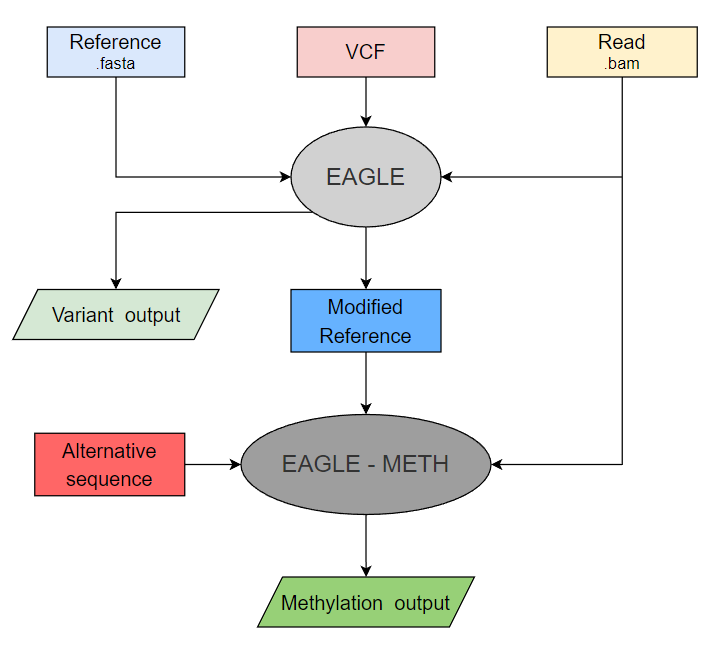
\includegraphics[scale=0.8]{figures/eagle_workflow_v2.PNG}
  \caption{EAGLE-METH workflow}
  \label{fig:EAGLE-METH}
\end{figure}

\subsection{Genome reference}
First, according to the original EAGLE, we know that EAGLE will output the variant set that best matches the given sequence. Therefore, we run the original EAGLE once, select the most compatible variant set, take these variant sites as the standard, and modify our reference so that it is modified to include the variant case. So we get a new modified reference sequence (figure 6. the blue rectangular part).
\par This approach can help us to evaluate the forward strand C to T and the reverse strand G to A cases later on, without the changes of these bases affecting our assumptions and results, i.e. to handle cases like SNPs, which can help us to focus on searching for CpG methylation issues.
\subsection{Read information}
In our input file, in addition to the genome reference and the vcf file, there is also the read information. Unlike EAGLE, in the EAGLE-METH framework, our reads must be bisulfite-treated and must contain both variant and methylation information. In our experiments, we use the simulated bisulfite sequencing results, and the FASTQ file generated by the MethylFASTQ tool is processed by different genetic sequencing tools to conform to the EAGLE-METH input format.
\par First, we use the BWA-meth tool to pre-process the FASTQ file, mapping the reference genome sequence we want to input with the read, and generating a SAM file from the mapping result. Then, we use the SAMtools tool, because the SAM file generated by BWA-meth is not in binary format, so we use SAMtools to convert it to a BAM file, and after converting it to the BAM file, we do the file sort, and the given index action. The processed BAM file is the one that contains the forward strand and the reverse strand information. In the EAGLE-METH probability model, we have to deal with the forward strand and reverse strand in the BAM file. When the calculated read is the forward strand, we need to pay attention to the C to T case; conversely, when the calculated read is the reverse strand case In the case of G to A, it is necessary to deal with the case of G to A (see figure \ref{fig:EAGLE-METH} the yellow rectangular part).
\subsection{Hypothetical sequences}
In EAGLE-METH, two different Hypothetical sequences are also given.
The first one is the hypothetical reference sequence, and we will use the previously introduced modified reference sequence in order to compare the calculated probability with different reads. If the 'C' position of the forward strand is replaced by the letter 'M', and the 'C' position of the reverse strand is replaced by the letter 'W'. The new reference is to enter the Hypothetical reference of EAGLE-METH, so the set of letters has been expanded and the current nucleotide bases set has been changed to A, T, C, G, M, W. The second is the hypothetical alternative sequence. In EAGLE-METH, when we determine the methylation sites to be calculated each time, we will divide the neighboring methylation sites into different subsets, and before each input model calculation, we will do a combination of each subset to consider the possibility of each different methylation. We will consider the possibility of each methylation hypothesis because we believe that the occurrence of DNA methylation may be affected by the neighboring methylation. Therefore, each different methylation site hypothesis is a hypothetical situation that occurs independently, which is our alternative sequence (see figure \ref{fig:meth_set}).

\begin{figure}[h]
  \centering
  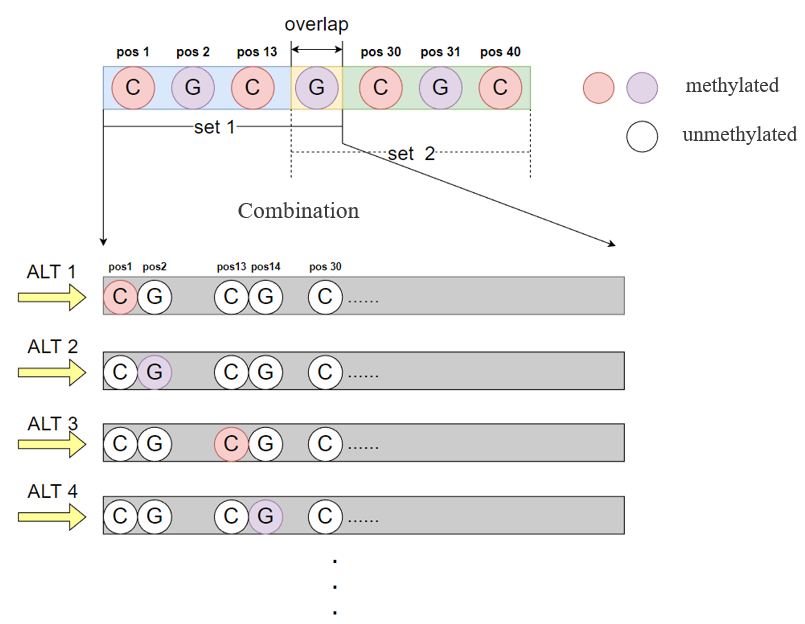
\includegraphics[scale=0.8]{figures/meth_set_v2.PNG}
  \caption{How methylation set do combination to produce the alternative sequence}
  \label{fig:meth_set}
\end{figure}
\vfill
\vfill
\subsection{Calculate marginal probability}
The probability model of EAGLE-METH is based on EAGLE's calculation algorithm (see figure \ref{fig:ref} and \ref{fig:alt}), which calculates two different hypothetical sequences separately and selects the probability with higher likelihood. In EAGLE-METH, we need to take into account the different situations of the forward strand and the reverse strand. Therefore, there will be different calculation probabilities, and handle the C to T of the forward strand and the G to A of the reverse strand respectively. The original probability table based on the quality score is modified into a probability matrix that conforms to the bisulfite sequence.
\begin{figure}[h!]
  \centering
  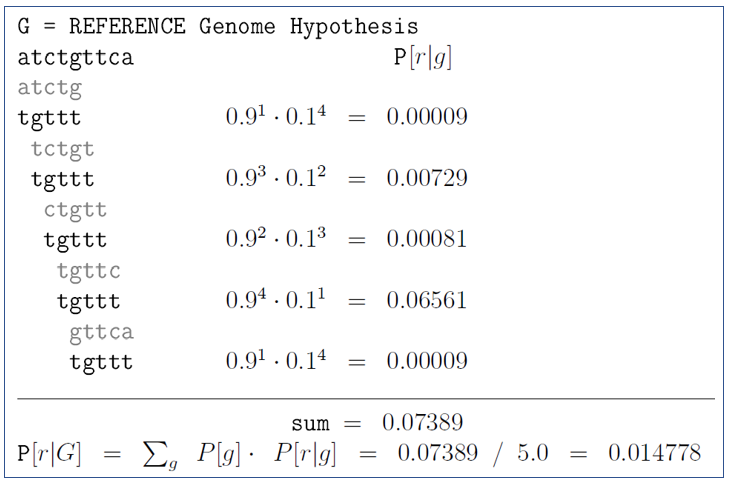
\includegraphics[scale=0.8]{figures/ref.PNG}
  \caption{The hypothetical reference sequences calculate in EAGLE}
  \label{fig:ref}
\end{figure}
\begin{figure}[h!]
  \centering
  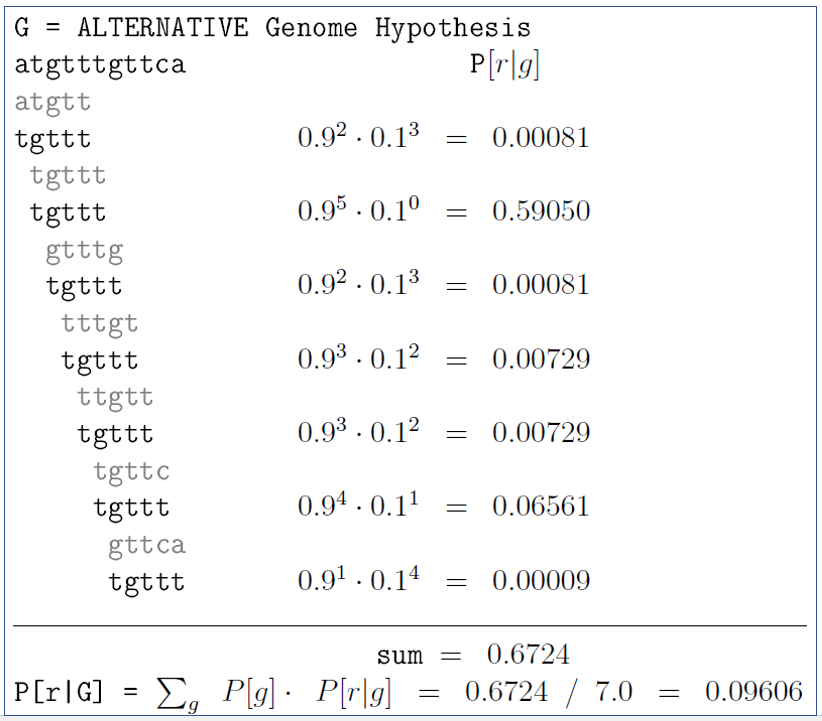
\includegraphics[scale=0.6]{figures/alter.PNG}
  \caption{The hypothetical alternative sequences calculate in EAGLE}
  \label{fig:alt}
\end{figure}
The calculation process is to first cut the reference into small regions and calculate one region at a time instead of calculating the whole reference sequence at once.
Then, we continue the previous content section 3.2.3, we assume each combination into a different alternative sequence and use the Greedy algorithm to keep the maximum value after each likelihood calculation, and finally use the maximum value as the final value of our alternative sequence. And this result is used to compare with the value of the reference sequence to select the one with higher likelihood probability, which is the calculation process of EAGLE-METH.
\par The final output of EAGLE-METH is the .tab file including methylation probability information (see Figure \ref{fig:output} ), and it retains the variant evaluation function of the original EAGLE, outputting a variant evaluation file. Some important fields are: chromosome ID field represents the chromosome from which the target of the experiment is chromosome; 
The reference base field and alternative base field represent the site where the methylation occurred, and this methylation is indicated by 'M' if it is from the forward strand, and 'W' if it is from the reverse strand; 
Reads field represents the total number of reads pile-up to this position; Marginal probability represents the probability calculated by EAGLE-METH, which represents the probability of methylation of 'C' / (probability of methylation of 'C' + probability of non-methylation of 'C') if the value is higher, it means that the methylation level is higher, and conversely, the lower the methylation level is.
\begin{figure}[h]
  \centering
  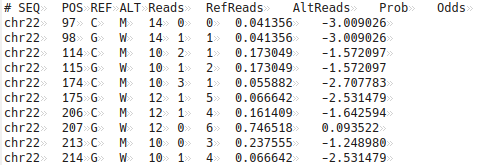
\includegraphics[scale=0.8]{figures/output_example.PNG}
  \caption{The EAGLE-METH output format example}
  \label{fig:output} 
\end{figure}
\par We believe that by extending the original EAGLE probability model and modifying its computational model to take into account bisulfite treated and methylation properties, we can also obtain a tool for both genetic variant evaluation and DNA methylation sites occurrence evaluation.

% \subsection{Likelihood Calculation}
% Our model assumes the data follows a standard normal distribution $𝒩(μ,σ²)$, so the likelihood function is:

% \begin{align*}
% ℒ  \;=&\;\;  \frac{1}{σ\sqrt{2π}}\, \exp\Big( \frac{-(x-μ)²}{2σ²}\Big)\\[.5ex]% .5ex adds extra vertical height
%      ∝&\;\;  σ⁻¹\, \exp\big( -½\,z²)  \hspace{1cm} \text{where~~} z ≝ \frac{x-μ}{σ}
% \end{align*}



% \begin{table}
% \begin{tabularx}{0.9\linewidth}{lX}
% Notation                                               &  Description\\
% \toprule
% $P_{\text{meth}\,|\,\textsf{context,BG}}$                    &  The background probability of methylation by context.\\[.3ex]
% $n_{\textsf{context},\,i}$                                 &  The number of cytosines (with sufficient read coverage)\newline of the given context occurring at position $i$ in the set of TFBS.\\[.3ex]
% $\overline{v}\,|\,\scriptstyle{\textsf{context},i}$  & The average methylation values of those cytosines.\\
% \bottomrule
% \end{tabularx}
% \caption{Summary of notation used in this thesis.}
% \label{tab:notation}
% \end{table}

% \section{Proposed Scheme}
% Write a bunch of stuff here.

	
\chapter{Experiment and Results}
In this chapter, we will present several experiments with the EAGLE-METH tool in practice.
\section{Environment}
In the EAGLE-METH experiment, we used the MethylFASTQ that can flexibly simulate bisulfite-treated data and some tools to process biological genetic information.

\begin{figure}[h]
  \centering
  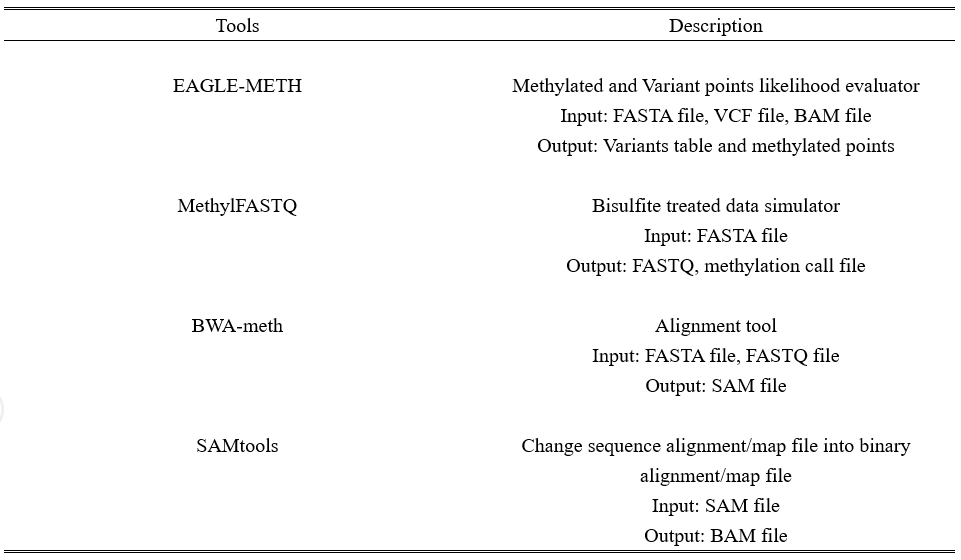
\includegraphics[scale=0.8]{figures/Table1.PNG}
  \caption{Experiment configuration}
  \label{fig:Experiment_configuration} 
\end{figure}
\par For the EAGLE-METH experiment, the human GRCh37 chromosome 22 fragment and the Arabidopsis chromosome M fragment were used to simulate the bisulfite-treated sequences and a methylation call file by MethylFASTQ. The results were evaluated by EAGLE-METH at different methylation levels and different species to compare whether the results were close to the correct methylation call file.
\section{Experiment}
\begin{figure}[h]
  \centering
  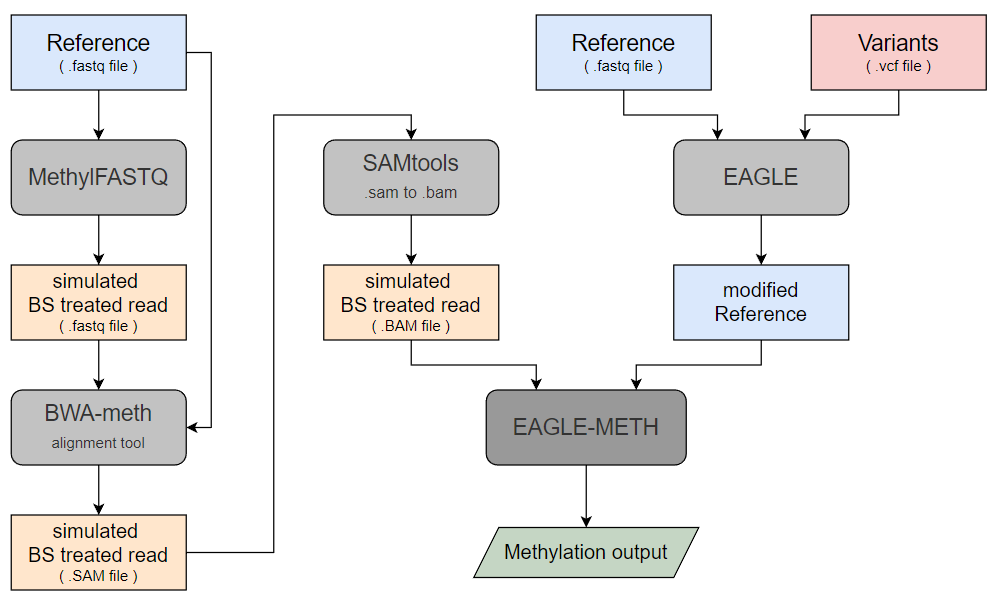
\includegraphics[scale=0.8]{figures/experiment_workflow_v2.PNG}
  \caption{Workflow of my experiment}
  \label{fig:exp_Workflow} 
\end{figure}
\par Figure \ref{fig:exp_Workflow} shows the main flow of our experiment, processing each of the three main inputs of our EAGLE-METH. First, see the left part of Figure \ref{fig:exp_Workflow}, we use MethylFASTQ to process the target reference genome fragment of interest. Then we use BWA-meth, an alignment tool, to pre-process the simulated reads, align the reads with the reference genome and generate a SAM file. SAMtools is used to process the file format and convert the SAM file to a BAM file, which can be used as the input of EAGLE-METH. In addition, in the right part of Figure \ref{fig:exp_Workflow}, we convert the information of candidate variants. That is, the red area and the reference genome, to the sites with the highest possibility of variant occurrence using EAGLE, and get a sequence that has finished processing the variant sites, namely modified reference, which can reduce the possibility of being affected by variants when doing methylation calculation later.
\par Finally, the read BAM file and the modified reference will be input into EAGLE-METH for calculation, and the above is the process of our experiment.

\begin{table}[h!]
  \renewcommand\arraystretch{2}
	\centering
	\begin{tabular}{l*{5}{c}}
    \hline
		Data              & Description\\
		\hline
		Chr 22 & GRCh37 chromosome 22, fragment of 27920bp  \\
		Chr M  & Arabidopsis chromosome M, fragment of 19530bp  \\
    \hline
	\end{tabular}
	\caption{Experiment Data}
	\label{table:1}
\end{table}
\par In our experiments, we used two different species of gene fragments, one of which is GRCh37 from the human genome database, and selected chromosome 22 to retrieve the target fragment. The other one is the chromosome M of Arabidopsis, and the target fragment was also extracted.

\begin{figure}[h]
  \centering
  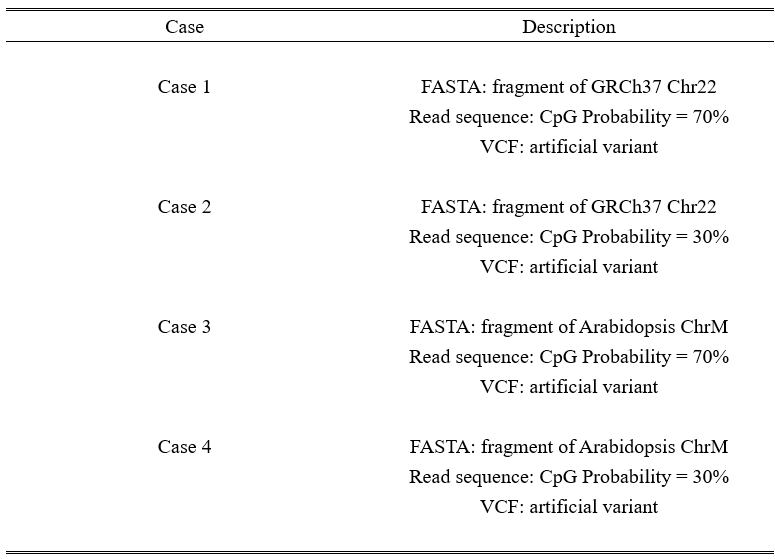
\includegraphics[scale=0.8]{figures/Table3.PNG}
  \caption{Different cases in our experiment}
  \label{fig:cases} 
\end{figure}
\par As you can see in Figure \ref{fig:cases}, there are four different cases in our experiment. The human chromosome GRCh37 chromosome 22 and Arabidopsis chromosome M were simulated by MethylFASTQ at two different levels of DNA methylation, CpG=30\%, and CpG=70\%, and the experimental results are shown below:
\vspace{15mm}
\begin{table}[h!]
	\centering
	\begin{tabular}{l*{5}{c}}
		Position    & REF & ALT & Strand & Marginal Probability & Methylation Level\\
		\hline
		99  & G & W & - & 0.56 & 0.5  \\
		213 & C & M & + & 0.78 & 0.86  \\
		634 & G & W & - & 0.58 & 0.57  \\
		688 & C & M & + & 0.83 & 0.8  \\
		689 & G & W & - & 0.11 & 0.6  \\
    703 & C & M & + & 0.68 & 0.75  \\
		822 & G & W & - & 0.54 & 0.5  \\
    1245 & C & M & + & 0.68 & 0.62  \\
	\end{tabular}
	\caption{The EAGLE-METH output of case 1}
	\label{case_1}
\end{table}

\begin{figure}[h!]
  \centering
  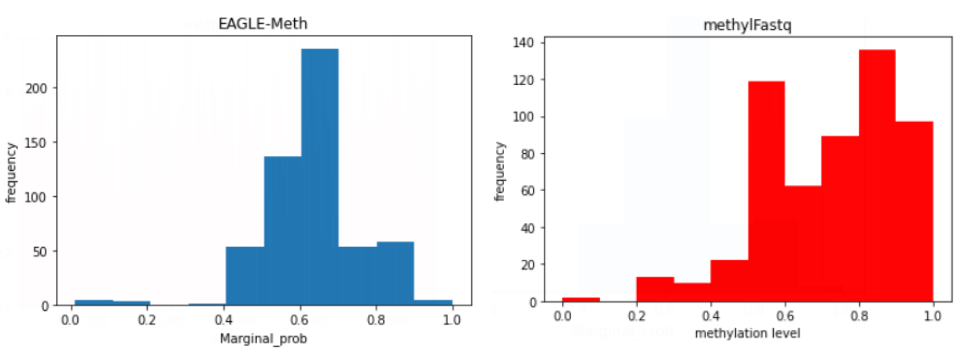
\includegraphics[scale=0.8]{figures/CHR22_70.PNG}
  \caption{Case 1 (chr22 CpG=70\%) distribution of the frequency of methylation level}
  \label{fig:case_1_1} 
\end{figure}
\begin{figure}[h!]
  \centering
  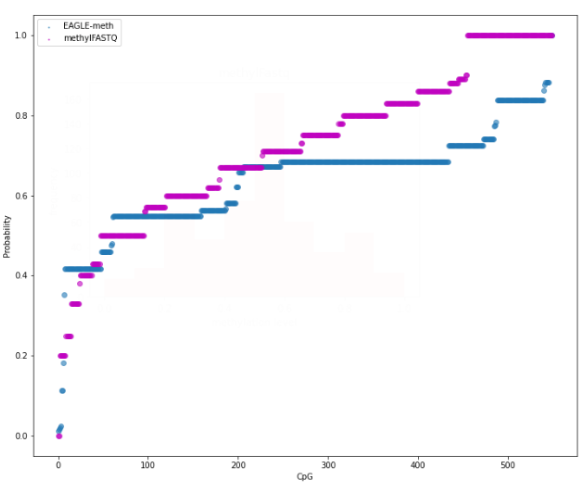
\includegraphics[scale=0.8]{figures/CHR22_70_2.PNG}
  \caption{Case 1 (chr22 CpG=70\%) sorted of CpG' probability}
  \label{fig:case_1_2} 
\end{figure}

\par According to Table \ref{case_1}, we can find that in the case1, with the fragment of Chr22 and the methylation level of CpG at 70\%, the Marginal probability calculated by EAGLE-METH and the methylation call file generated by the MethylFASTQ file, we can find that the calculation result of EAGLE-METH is close to the methylation call file.
In addition, we can see that in Figure \ref{fig:case_1_1} and \ref{fig:case_1_1}, we have calculated the probability frequency of each occurrence in different probability cases, and from the figure, we can also find that the statistical quantity of blue EAGLE-METH falls in 0.6 to 0.8, and the statistical quantity of the red part, the methylation level of MethylFASTQ falls between 0.5 and 0.9. It can be found that the results of EAGLE-METH are more concentrated, but the evaluation results are also close to the correct answers.
\par In figure \ref{fig:case_1_2},we also compared the results of the two tools by ranking the probability of each CpG site from small to large. The red line is MethylFASTQ and the blue line is EAGLE-METH, we can find that the results of the two tools are close to each other.
\vspace{15mm}
\begin{table}[h!]
	\centering
	\begin{tabular}{l*{5}{c}}
		Position    & REF & ALT & Strand & Marginal Probability & Methylation Level\\
		\hline
		213  & C & M & + & 0.17 & 0.2  \\
		214 & G & W & - & 0.15 & 0.2  \\
		633 & C & M & + & 0.16 & 0.2  \\
		634 & G & W & - & 0.35 & 0.4  \\
		703 & C & M & + & 0.76 & 0.14  \\
    704 & G & W & - & 0.15 & 0.14  \\
		1296 & G & W & - & 0.16 & 0.12  \\
    1645 & G & W & - & 0.44 & 0.4  \\
	\end{tabular}
	\caption{The EAGLE-METH output of case 2}
	\label{case2}
\end{table}

\begin{figure}[h!]
  \centering
  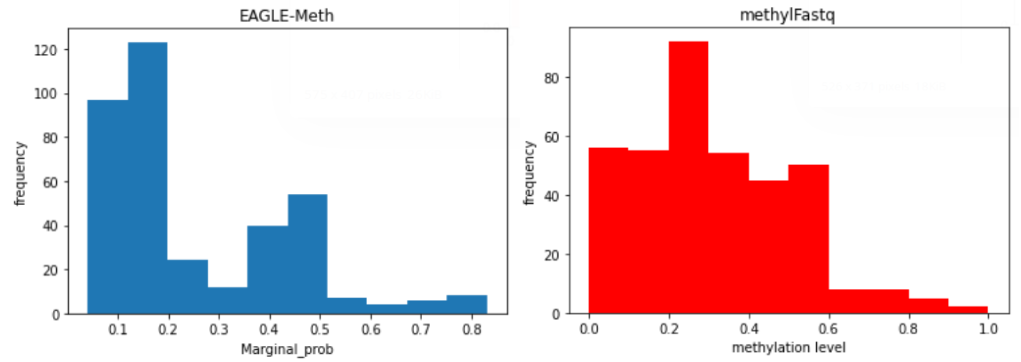
\includegraphics[scale=0.8]{figures/CHR22_30.PNG}
  \caption{Case 2 (chr22 CpG=30\%) distribution of the frequency of methylation level}
  \label{fig:case_2_1} 
\end{figure}
\begin{figure}[h!]
  \centering
  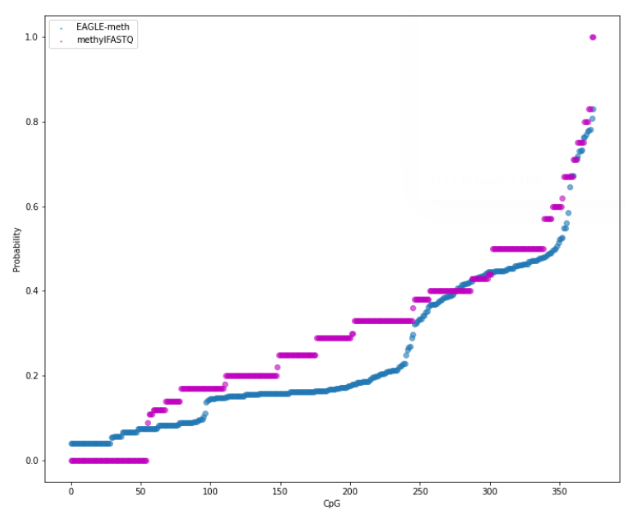
\includegraphics[scale=0.8]{figures/CHR22_30_2.PNG}
  \caption{Case 2 (chr22 CpG=30\%) sorted of CpG' probability}
  \label{fig:case_2_2} 
\end{figure}

\par According to Table \ref{case2}, in case2, the fragment of Chr22 and the methylation level of CpG is 30\%, we can find that the calculation result of EAGLE-METH is quite close to the methylation call file. In addition, we can see Figure \ref{fig:case_2_1}, from the figure, we can find that the statistical quantity of blue EAGLE-METH mainly falls in the range of 0 to 0.3. Similarly, the statistical quantity of the methylation level of MethylFASTQ in the red part falls in the range of 0 to 0.5. It can be found that the results of EAGLE-METH are still more concentrated, but the evaluation results are also close to the correct answers. 
\par We also compared the results of the two tools in figure \ref{fig:case_2_2}, by ranking the probability of each CpG site from small to large. The red line is MethylFASTQ and the blue line is EAGLE-METH.
% \vfill
\vspace{15mm}
\begin{table}[h!]
	\centering
	\begin{tabular}{l*{5}{c}}
		Position    & REF & ALT & Strand & Marginal Probability & Methylation Level\\
		\hline
		37  & C & M & + & 0.7 & 0.8  \\
		38 & G & W & - & 0.57 & 0.6  \\
		122 & C & M & + & 0.52 & 0.43  \\
		123 & G & W & - & 0.54 & 0.62 \\
		240 & C & M & + & 0.7 & 0.62  \\
    241 & G & W & - & 0.59 & 0.62  \\
		565 & C & M & + & 0.96 & 1  \\
    566 & G & W & - & 0.96 & 1  \\
	\end{tabular}
	\caption{The EAGLE-METH output of case 3}
	\label{case3}
\end{table}

\begin{figure}[h!]
  \centering
  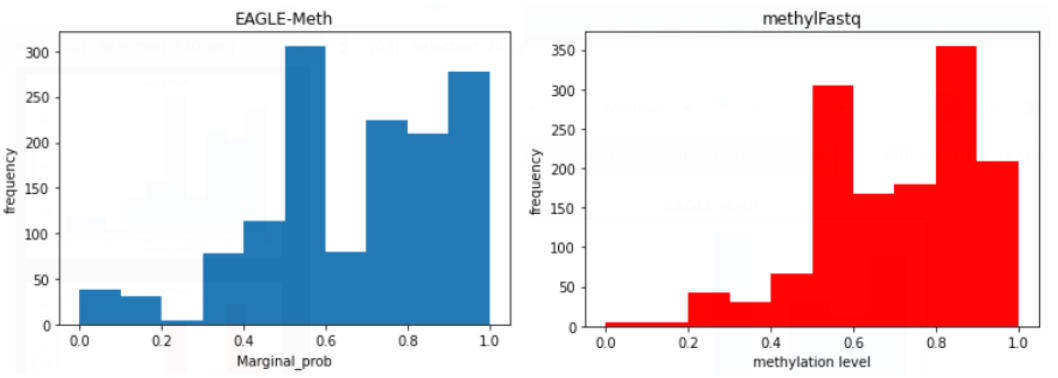
\includegraphics[scale=0.8]{figures/CHRM_70.PNG}
  \caption{Case 3 (chrM CpG=70\%) distribution of the frequency of methylation level}
  \label{fig:case_3_1} 
\end{figure}
\begin{figure}[h!]
  \centering
  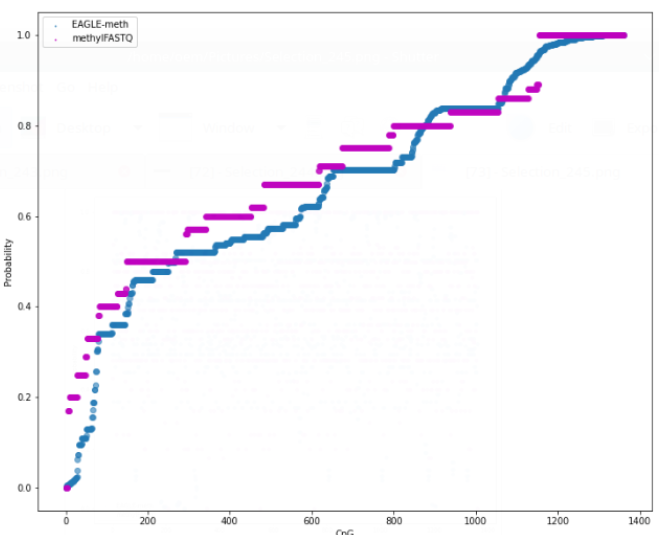
\includegraphics[scale=0.8]{figures/CHRM_70_2.PNG}
  \caption{Case 3 (chrM CpG=70\%) sorted of CpG' probability}
  \label{fig:case_3_2} 
\end{figure}

\par According to Table \ref{case3}, in case3, the fragment of ChrM and the methylation level of CpG is 70\%. And we can find that the calculation result of EAGLE-METH is quite close to the methylation call file. See figure \ref{fig:case_3_1}, the statistical quantities of EAGLE-METH in blue are mainly concentrated in 0.5 and between 0.7 to 1, and the statistical quantities of the methylation level of MethylFASTQ in red fall in the range of 0.5 to 1. In figure \ref{fig:case_3_2}, we also ranked the probability of each CpG site from small to large and compared the results of the two tools.  It can be found that they are also close to each other.

\vspace{15mm}
\begin{table}[h!]
	\centering
	\begin{tabular}{l*{5}{c}}
		Position    & REF & ALT & Strand & Marginal Probability & Methylation Level\\
		\hline
		37  & C & M & + & 0.17 & 0.25  \\
		123 & G & W & - & 0.06 & 0  \\
		130 & C & M & + & 0.17 & 0.6  \\
		131 & G & W & - & 0.16 & 0.2 \\
		197 & C & M & + & 0.34 & 0.29 \\
    198 & G & W & - & 0.09 & 0  \\
		383 & C & M & + & 0.18 & 0.22  \\
    384 & G & W & - & 0.26 & 0.22  \\
	\end{tabular}
	\caption{The EAGLE-METH output of case 4}
	\label{case4}
\end{table}

\begin{figure}[h!]
  \centering
  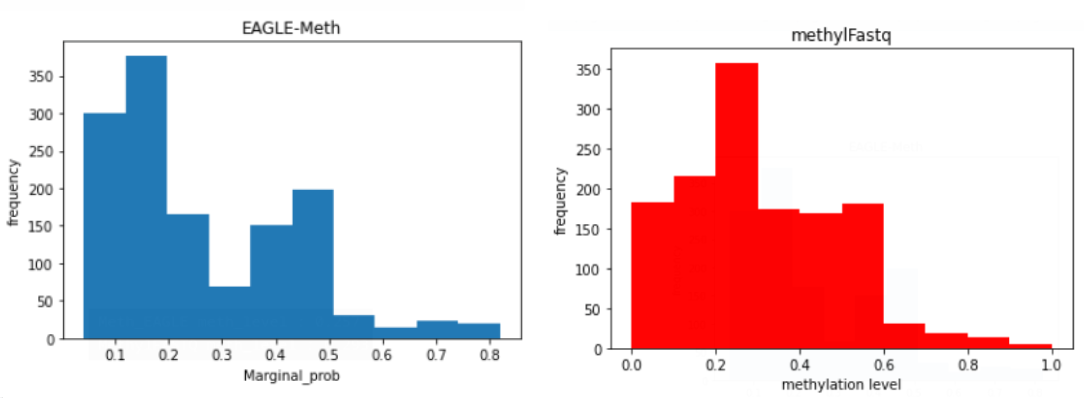
\includegraphics[scale=0.75]{figures/CHRM_30.PNG}
  \caption{Case 4 (chrM CpG=30\%) distribution of the frequency of methylation level}
  \label{fig:case_4_1} 
\end{figure}
\begin{figure}[h!]
  \centering
  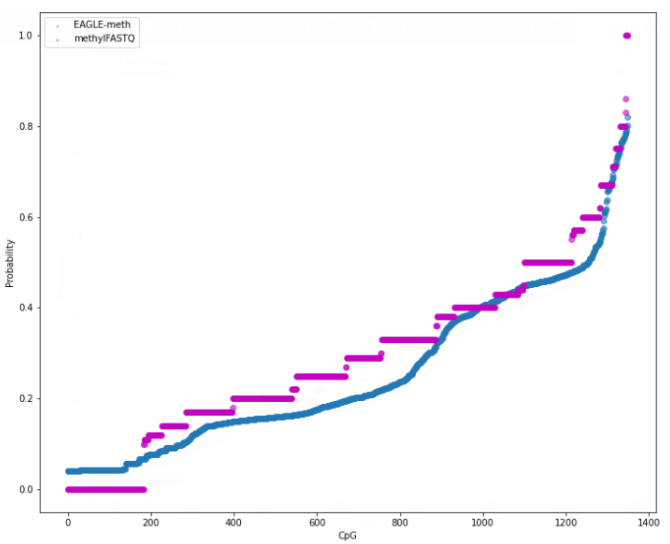
\includegraphics[scale=0.8]{figures/CHRM_30_2.PNG}
  \caption{Case 4 (chrM CpG=30\%) sorted of CpG' probability}
  \label{fig:case_4_2} 
\end{figure}
\vfill
\par According to Table \ref{case4}, in case4, the fragment of ChrM and the methylation level of CpG is 30\%, so we can find that the calculation result of EAGLE-METH is quite close to the methylation call file.
See figure \ref{fig:case_4_1}, the blue EAGLE-METH statistics mainly focus on 0 to 0.3 and the average falls on 0 to 0.5, while in the red part, the statistics of the methylation level of MethylFASTQ mainly falls on 0.3 and the average falls on 0~0.5. Figure \ref{fig:case_4_2}, The red line is for MethylFASTQ and the blue line is for EAGLE-METH. It can be found that they are still quite close.

\begin{figure}[h]
  \centering
  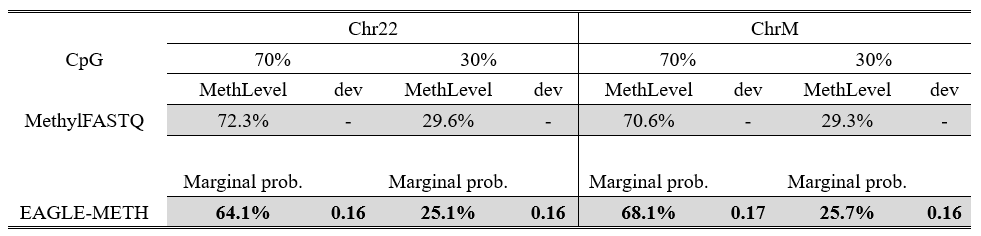
\includegraphics[scale=0.8]{figures/result.PNG}
  \caption{Each of case methylation level and average of each position deviation}
  \label{re} 
\end{figure}

\par Finally, we see Figure \ref{re}, the table mainly statistics Case1 to Case4 results. In case1, the average marginal probability output of EAGLE-METH is 64.1\% in 70\% simulated case, and the difference with the average 72.3\% of MethylFASTQ is about 8.2\%; In case2, the average marginal probability output of EAGLE-METH is 25.1\% at 30\% simulated, which is about 4.5\% different from the average 29.6\% of MethylFASTQ;   In case3, the average marginal probability output of EAGLE-METH is 68.1\% at 70\% simulated, which is about 2.5\% different from the average 70.6\% of MethylFASTQ; In case4, the average marginal probability output of EAGLE-METH is 25.7\% at 30\% simulated, which is about 3.6\% different from the average of 29.3\% for MethylFASTQ.
Moreover, from the table, it can be seen that for four different cases, the average difference between each position of EAGLE-METH and the position corresponding to the methylation call file of MethylFASTQ is calculated by subtracting the absolute value and the average value can be found to be around 16\%.



\chapter{Conclusion and Future work}
After analyzing the results of the experiments, we believe that EAGLE-METH can evaluate the occurrence of DNA methylation through its probability model, inputting the reference genome, the vcf, and the bisulfite-treated read, and comparing the results with the correct answers through simulated data, so we believe that the extension of EAGLE-METH is worthwhile. Therefore, we believe that the development of EAGLE-METH, a DNA methylation assessment system, is of research value. However, there are still some issues we can improve. For instance, the total calculation time. Because the reference genome sequence is very long data, and we are using the Greedy algorithm to do the calculation, it will cause the calculation time to be too long. Also, the lack of RAM is the reason that we can only calculate fixed-length regions at present.

\newpage
\AddToContents{Bibliography}
\printbibliography


\end{document}
